
\section{The \BaFePAs series}

The \BaFeAsP series progresses from \BaFeAs which becomes antiferromagnetic at around \unit[138]{K} and \BaFeP which is metallic to low temperatures. Neither end members are superconducting, however as arsenic is substituted for phosphor, the low temperature antiferromagnetic state decays, giving way to superconductivity which kicks in at approximately $x=0.18$ and increases to the optimal substitution of $x=0.31$ and then decreases until it gives way to a paramagnetic ground state at around $x=0.71$. \Fig\ref{Fig:3:PhaseDiagram} shows the phase diagram adapated ref. \cite{Nakai2010a} as determined by resistivety measurements.

\begin{figure}
    \begin{center}
        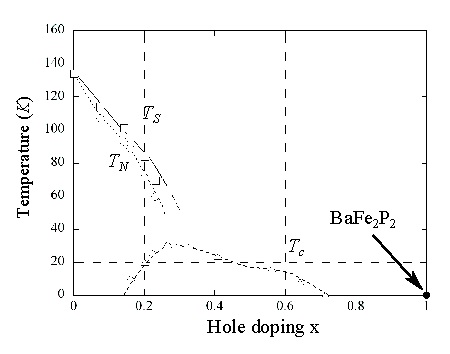
\includegraphics[scale=0.7]{Chapter3-dHvABaFe2P2/Figures/BaFe2P2Series/PhaseDiagram/PhaseDiagram}
        \caption{Phase diagram adapted from ref \cite{Nakai2010a} measured by resistivity. $T_s$, $T_N$ and $T_c$ are the structural transition, the antiferromagnetic transition and the superconducting transition temperatures respectively.}
        \label{Fig:3:PhaseDiagram}
    \end{center}
\end{figure}


The \BaFePAs series has been previously measured by members of the group at Bristol using dHvA oscillations\cite{Shishido2010}. The electron surfaces have been characterised for x ranging from $0.41$ to $1$ and have clearly shown that the DFT calculations consistently overestimate the size of the surfaces. Moreover, dHvA measurements on the material with $x=0.63$ have been performed where one of the hole sheets was observed\cite{Analytis2010c}.
